
% Autores:
%
%   FERNANDO LEANDRO FERNANDES
%   PEDRO DE CASTRO GURGEL LIMA
 

%%%%%%%%%%%% STRUCTURE %%%%%%%%%%%%%%%
\documentclass[12pt,a4paper]{article}
\usepackage[utf8]{inputenc}
\usepackage[portuguese,brazil]{babel}
\usepackage[T1]{fontenc}
\usepackage{amsmath}
\usepackage{amsfonts}
\usepackage{amssymb}
\usepackage{makeidx}
\usepackage{graphicx}
\usepackage[left=2cm,right=2cm,top=2cm,bottom=2cm]{geometry}
\usepackage{lmodern}
\usepackage{setspace}
\usepackage{subfig}
\usepackage{mathptmx}
\usepackage{changepage}
\usepackage{epstopdf}
\usepackage{enumerate}

%%%%%%%%%%%% PAGES STYLE %%%%%%%%%%%%%
\usepackage{fancyhdr}
\fancypagestyle{main}{
\renewcommand{\headrulewidth}{0pt}
\fancyhead[RO]{\thepage}
\fancyfoot[CO]{}
}

%%%%%%%%%%% PDF METADATA %%%%%%%%%%%%%
\usepackage[pdfauthor={
FERNANDO LEANDRO FERNANDES,
PEDRO DE CASTRO GURGEL LIMA},
pdftitle={RELATÓRIO DA 1\textordfeminine EXPERIÊNCIA},
pdfsubject={ALGORITMOS GENÉTICOS N-RAINHAS},
pdfkeywords={n-rainhas,AG,DCA,IA},
hidelinks]{hyperref}

%%%%%%%%%%%%%%%% CODE %%%%%%%%%%%%%%%%
\usepackage{listings}
\lstset{
 %% Escape para comentários:
 %% /*Comentário*/
 language=Python,
 extendedchars=\true,
 inputencoding=utf8,
 literate=%
  {*}{{\**}}1
  {-}{{\--}}1,
 escapeinside={/*}{*/},
 texcl=\true,
 commentstyle=\it,
 stringstyle=\bf,
 belowcaptionskip=5pt,
 numbers=left, 
 stepnumber=1,
 firstnumber=1,
 tabsize=2,
 numberstyle=\tiny, 
 breaklines=true,
 frame=tb,
 basicstyle=\footnotesize,
 stringstyle=\ttfamily,
 showstringspaces=false,
 morekeywords={PALAVRAS,RESERVADAS-DA-LINGUAGEM}, 
}

\begin{document}
\onehalfspacing
\thispagestyle{empty}
\setcounter{page}{1}

%%%%%%%%%%%%%% LOGOS %%%%%%%%%%%%%%%%
\begin{figure}[!ht]

\centering

\subfloat{

\includegraphics[width=2.7cm]{UFRN.jpg}
\label{UFRN Logo}
}
\hspace{11.09cm}
\subfloat{

\includegraphics[width=2.4cm]{DCA.jpg}
\label{DCA Logo}
}
\end{figure}

%%%%%%%%%%%%%%% CAPA %%%%%%%%%%%%%%%%%

\begin{center}
\vspace{-0.5cm}

{\bf{\normalsize UNIVERSIDADE FEDERAL DO RIO GRANDE DO NORTE\\
CENTRO DE TECNOLOGIA\\
DEPARTAMENTO DE ENGENHARIA DE COMPUTAÇÃO E AUTOMAÇÃO\\
CURSO DE ENGENHARIA DE COMPUTAÇÃO
}}

\vspace{3.6cm}

{\bf{\large RELATÓRIO DA 2\textordfeminine\phantom{a}EXPERIÊNCIA\\
RESOLUÇÃO DAS N-RAINHAS COM ALGORITMOS GENÉTICOS (N-Generation)\\
}}

\vspace{4cm}

\begin{flushright}
\begin{normalsize}
FERNANDO LEANDRO FERNANDES:20150146106\\
\vspace{0.6cm}
PEDRO DE CASTRO GURGEL LIMA:2008020576\\

\end{normalsize}
\end{flushright}

\vspace{7cm}

{\large Natal-RN\\
2016}


\end{center}

%%%%%%%%%%%%% CONTRA-CAPA %%%%%%%%%%%%
\newpage
\thispagestyle{empty}

\begin{center}
\begin{normalsize}
FERNANDO LEANDRO FERNANDES:20150146106\\
\vspace{0.6cm}
PEDRO DE CASTRO GURGEL LIMA:2008020576\\
\end{normalsize}
\end{center}
\vspace{3cm}

{\bf{\large {\centering RESOLUÇÃO DAS N-RAINHAS COM ALGORITMOS GENÉTICOS (N-Generation)\\}}}

\vspace{4cm}

\begin{adjustwidth}{7.5cm}{0cm}

{\normalsize

Primeiro Relatório apresentado à disciplina de
Inteligência Artificial Aplicada, correspondente à
avaliação da 1º unidade do semestre 2016.1 do curso de 
Engenharia de Computação e Automação da Universidade 
Federal do Rio Grande do Norte, sob orientação do 
{\bf Prof. Alan Robson Silva Venceslau.}

}

\end{adjustwidth}

\vspace{2cm}

\begin{center}

Professor: Alan Robson Silva Venceslau.

\vspace{6cm}

{\large Natal-RN\\
2016}

\end{center}

%%%%%%%%%%%%%%% RESUMO %%%%%%%%%%%%%%%%
\newpage
\thispagestyle{empty}

\begin{center}
{\large \textbf{RESUMO}}
\end{center}

\vspace{3cm}

\hspace{4ex}O presente trabalho apresenta uma aplicação de algoritmo genético para um problema clássico, n-rainhas, em que o posicionamento das peças e parâmetros do algoritmo são discutidos e apresentados baseados em pesquisas teóricas e expostos com uma interface amiga ao usuário.

\vspace{1.5cm}

\textbf{Palavras-chave: Algoritmos Genéticos, n-rainhas, geração, mutação, JAVA.}

%%%%%%%%% LISTA DE SÍMBOLOS %%%%%%%%%%%
%\newpage
%\thispagestyle{empty}
%
%\begin{center}
%{\large \textbf{LISTA DE SÍMBOLOS}}
%\end{center}
%
%\vspace{3cm}
%
%\begin{tabular}{ l l }
%$F_{in}$\hspace{1.5cm} & Vazão de entrada no tanque;\\
%\phantom{a} & \phantom{a}\\
%$K_m$\hspace{1.5cm} & Constante da bomba utilizada;\\
%\phantom{a} & \phantom{a}\\
%\end{tabular}

%%%% LISTA DE ABREVIATURAS E SIGLAS %%%%
\newpage
\thispagestyle{empty}

\begin{center}
{\large \textbf{LISTA DE ABREVIATURAS E SIGLAS}}
\end{center}

\vspace{3cm}

\begin{tabular}{ l l }
AG\hspace{1.5cm} & Abreviação para Algoritmo Genético.\\
\end{tabular}


%%%%%%%%%% LISTA DE FIGURAS %%%%%%%%%%
\newpage
\thispagestyle{empty}

\begin{center}
\listoffigures
\end{center}



%%%%%%%%%%%%%%% SUMÁRIO %%%%%%%%%%%%%%
\newpage
\thispagestyle{empty}
\begin{center}
\tableofcontents
\end{center}

%%%%%%%%%%%%% INTRODUÇÃO %%%%%%%%%%%%%
\newpage
\thispagestyle{main}

\section{INTRODUÇÃO}


\hspace{4ex}Baseados na teoria envolvida em sala de aula e por pesquisas feitas na internet, foi desenvolvido o programa \textbf{\emph{N-Generation}}, onde o problema das n-rainhas é tratado fazendo uso de algoritmo genético de forma auto-explicativa, apresentando dados de resposta em tela, através de gráficos e posicionamento das peças na malha quadriculada simulando o tabuleiro de Xadrez.


%%%%%%%%% REFERENCIAL TEÓRICO %%%%%%%%
\newpage
\thispagestyle{main}

\section{REFERENCIAL TEÓRICO}

\subsection{O que é algoritmo genético?}

\hspace{4ex}Um \textbf{algoritmo genético} (AG) nada mais é que uma técnica de busca utilizada na computação para achar soluções aproximadas em problemas de otimização e busca, fundamentado principalmente pelo americano John Henry Holland. Algoritmos genéticos são uma classe particular de algoritmos evolutivos que usam técnicas inspiradas pela biologia evolutiva como hereditariedade, mutação seleção natural e recombinação (ou \textit{crossing over}).

\subsubsection{Características}

\begin{itemize}
	\item AGs trabalham com uma codificação do conjunto de parâmetros e não com os próprios;
	\item AGs trabalham com uma população e não com um único ponto;
	\item AGs utilizam regras de transição probabilísticas e não determinísticas;
	\item AGs utilizam informações de custo ou recompensa e não derivadas ou outro conhecimento auxiliar.
\end{itemize}

\begin{figure}[!htb]
	\label{Figura 1}
	\centering
	\caption{Passos do Algoritmo Genético}
	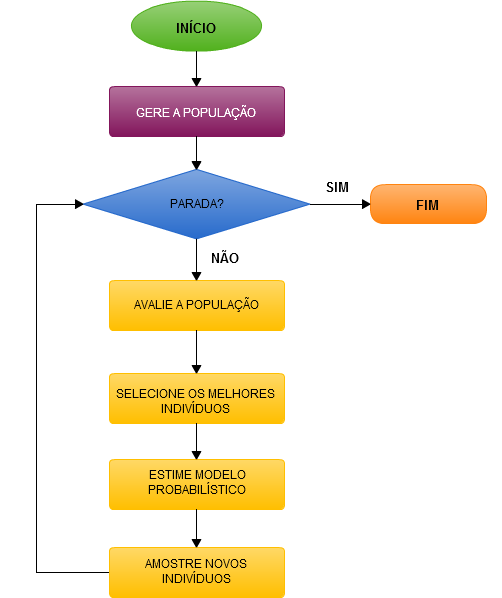
\includegraphics[width=10cm]{FLUXOGRAMA.png}
\end{figure}

\newpage
\thispagestyle{main}

\subsubsection{Aplicações}

\hspace{4ex}Dentre a vasta aplicabilidade devido a sua adaptabilidade, os algoritmos genéticos se apresentam muito bem em ambientes dinâmicos, onde essa flexibilidade proporcionada resulta em soluções satisfatórias como em:

\begin{itemize}
\item Controle de Sistemas Dinâmicos;
\item Indução e Otimização de Bases de Regras;
\item Encontrar Novas Topologias Conexionistas:
\item Engenharia de Sistemas Neurais Artificiais;
\item Modelagem de Estruturas Neurais Biológicas;
\item Simulação de Modelos Biológicos:
	\begin{itemize}
	\item Comportamento;
	\item Evolução;
	\end{itemize}
\end{itemize}


\subsubsection{População e o Indivíduo}

\hspace{4ex}A população será composta por todos os indivíduos de uma geração determinada onde ela deverá ser grande o suficiente para que a solução inicial possa realizar uma boa prospecção atrás de indivíduos com bom grau de aptidão (\textit{fitness}). Sendo a função objetivo em $R^2$, cada indivíduo será composto por um par ordenado de valores (x, y); Onde ambos possuirão representações cromossômicas independentes (um para x e outro para y).

\subsubsection{Aptidão ou Fitness e Elitismo}

\hspace{4ex}Foi adotado que a aptidão será medida utilizando o próprio indivíduo aplicado na função objetivo. Esse índice diz o quão bom é esse indivíduo ou não. Quando se é mantido o elitismo no procedimento, mantem-se uma quantidade fixa de pais na troca de gerações, propagando uma cópia dos melhores indivíduos para gerações posteriores.

\newpage
\thispagestyle{main}

\subsubsection{Seleção}

\hspace{4ex}O procedimento de seleção é um ponto chave no algoritmo, podendo ser realizado por torneio, roleta, ranking ou truncamento.

Seleção por Torneio:
\begin{itemize}
	\item Escolhe-se k (tipicamente 2) indivíduos aleatoriamente da população e o melhor é selecionado;
	\item Não é proporcional a aptidão;
	\item Não é necessário roda da roleta, escalamento da aptidão ou ranking.
\end{itemize}

Seleção por Roleta: Os indivíduos são ordenados de acordo com a função-objetivo e lhes são atribuídas probabilidades decrescentes de serem escolhidos - probabilidades essas proporcionais à razão entre a adequação do indivíduo e a soma das adequações de todos os indivíduos da população. A escolha é feita então aleatoriamente de acordo com essas probabilidades. Dessa forma conseguimos escolher como pais os mais bem adaptados, sem deixar de lado a diversidade dos menos adaptados. 

\subsubsection{Crossover \& Mutação}

\hspace{4ex}Crossover é um processo que imita o processo biológico homônimo na reprodução sexuada: os descendentes recebem em seu código genético parte do código genético do pai e parte do código da mãe. Esta recombinação garante que os melhores indivíduos sejam capazes de trocar entre si as informações que os levam a ser mais aptos a sobreviver, e assim gerar descendentes ainda mais aptos.\\

Por último vem as mutações, onde é verificado que poderá ocorrer em um indivíduo com boa aptidão, se tornando um indivíduo muito ruim, por isso se faz necessário o equilíbrio da taxa de mutação, não tão baixa que impeça a prospecção, mas também não tão alta que possa ocasionar divergência do ponto de mínimo (no nosso caso).


\newpage
\thispagestyle{main}

\subsection{N-rainhas (ou 8 rainhas)}

\hspace{4ex}Como é sabido, a rainha é a peça mais poderosa do xadrez, pois pode se movimentar em qualquer direção e por qualquer número de casas. Esse problema propõe colocar n rainhas (8 na dimensão de um tabuleiro clássico) em um tabuleiro de dimensão n, em uma certa posição que não ocorra nenhum ataque por nenhuma das peças. Por exemplo, em um problema com n=8, temos a seguinte configuração:\\

\begin{figure}[!htb]
	\label{Figura 2}
	\centering
	\caption{Solução para n=8}
	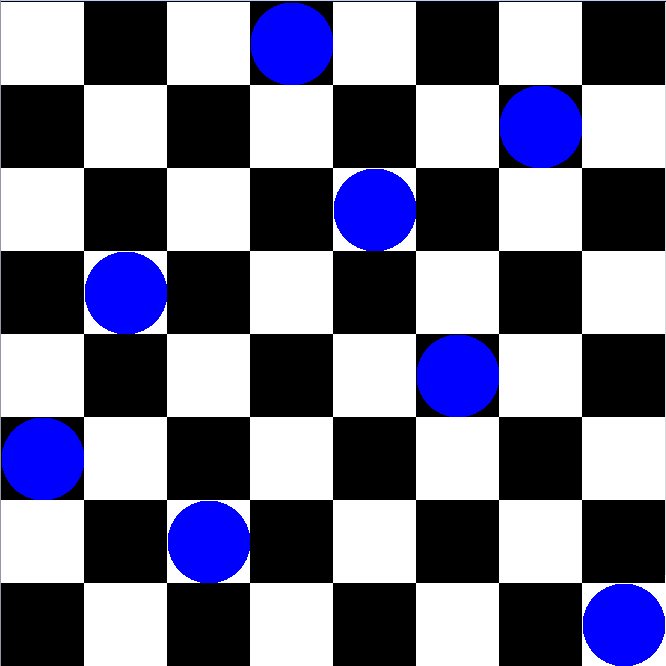
\includegraphics[width=6cm]{RAINHAS01.png}
\end{figure}

O tabuleiro acima seria representado pelo vetor \{5,3,6,0,2,4,1,7\}. Assim cada rainha é representada em uma coluna deste tabuleiro.
%%%%%%%%%% METODOLOGIA %%%%%%%%%%%%%%%
\section{METODOLOGIA}

\subsection{Implementação}

\hspace{4ex}A aplicação foi desenvolvida em JAVA\footnote{Mais em:http://www.oracle.com/technetwork/pt/java/javase/downloads/jdk8-downloads-2133151.html} em ambiente Eclipse\footnote{Mais em:https://eclipse.org/} juntamente com a API JfreeChart\footnote{Mais em:http://www.jfree.org/jfreechart/} para geração de gráficos, onde cada Indivíduo da população, representa uma possível solução, o gene é representado por um vetor de n posições, onde o índice do vetor é a posição x e o valor deste índice a posição y, de uma rainha no tabuleiro.

\newpage
\thispagestyle{main}

\subsection{Pacotes \& Classes}

A caráter de organização, o programa foi dividido em pacotes:

\begin{itemize}
\item evolução:
	\begin{itemize}
	\item Indivíduo;
	\item População;
	\item Tabuleiro. 
	\end{itemize}
\item genética:
	\begin{itemize}
	\item Execute.java
	\end{itemize}
\item GUI:
	\begin{itemize}
	\item AboutBox.java;
	\item Chart.java;
	\item Frame.java;
	\item PintaTabuleiro.java.
	\end{itemize}
\end{itemize}

\begin{enumerate}
\item \textbf{Indivíduo}: Classe que define uma possível solução, nela são implementados os métodos de adicionar rainha ao tabuleiro, avaliar as colisões e gerar aptidão a partir dessas colisões;
\item \textbf{População}: Classe que define um conjunto de indivíduos, atribuindo uma posição e ordenando-os dentro do vetor, tiramos a média de aptidão dos mesmos por: aptidão total/numero de indivíduos;
\item \textbf{Tabuleiro}: Classe que define o tabuleiro em um vetor bi-dimensional nxn, seus métodos de atualização e verificação das posições (livre ou ocupado);
\item \textbf{Execute}: Classe implementada com os métodos do AG, as operações de manipulação dos \textit{genes} (indivíduos) ocorrerão aqui, como: nova geração, \textit{crossover}, seleção (roleta/torneio), mutação e elitismo.
\item \textbf{AboutBox}: Método de interface para o "Sobre";
\item \textbf{Chart}: Método de interface implementado usando o \textit{JfreeChart} para gerar o gráfico de análise com o número de gerações x número de colisões;
\item \textbf{Frame}: Método principal de interface feito em Swing\footnote{Ver mais em: https://pt.wikipedia.org/wiki/Swing\_Java}, onde são expostos os gráficos/tabuleiro em abas, os campos para alteração dos parâmetros e tela de log para análise mais detalhada das operações.
\item \textbf{PintaTabuleiro}: Método de interface que modela o tabuleiro quanto a seus quadrados e peças (rainhas) nele.


\end{enumerate}


%%%%%%%%%%%%% CONCLUSÃO %%%%%%%%%%%%%%
\newpage
\thispagestyle{main}

\section{CONCLUSÃO}

\subsection{Resultados Obtidos}

\hspace{4ex} Aqui fica demonstrado algumas configurações de testes realizados, variando-se o tamanho de população, as taxas de mutação e crossover. É notado durante esses testes que ao se aumentar a quantidade de indivíduos na população ocorre maior taxa de sucesso e convergência mais rápida para o resultado, em menos gerações que o limite total, mesmo se aplica caso a população seja fixa e se aumente a taxa de mutação, aumentando assim a variabilidade genética dos indivíduos com ou sem o uso do elitismo, mas piorando visivelmente a aptidão média. Também foi visto que com taxas de crossover acima de 70\% responde melhor o algoritmo.\\

\subsubsection{Variação de População}

\begin{figure}[!htb]
	\label{Figura 3}
	\centering
	\caption{População = 100}
	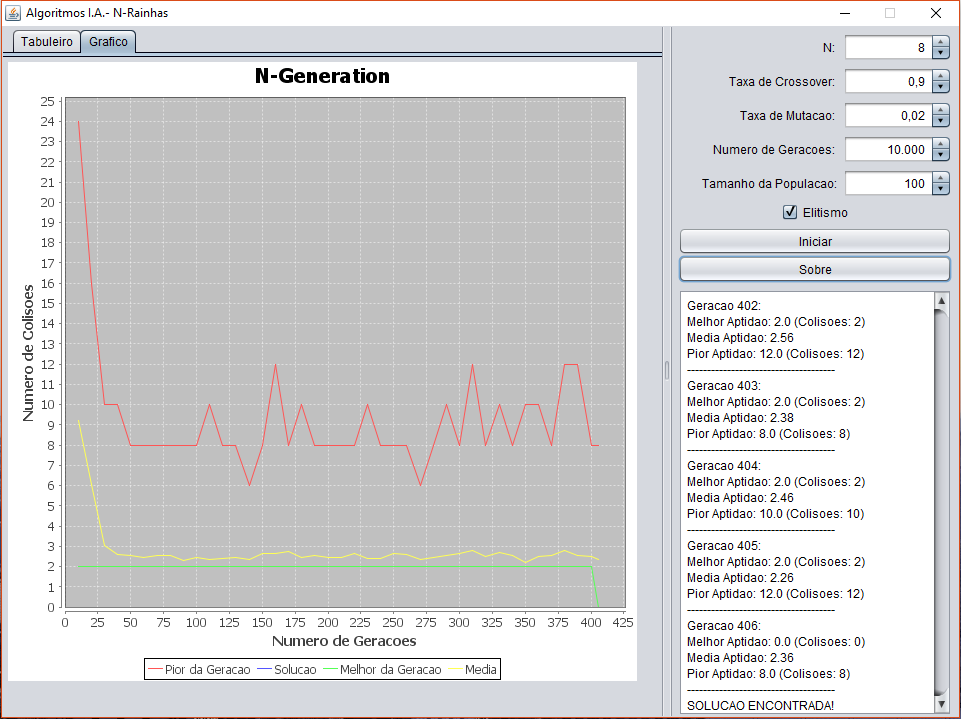
\includegraphics[width=14cm]{TELA01.png}
\end{figure}

\newpage
\thispagestyle{main}
\begin{figure}[!htb]
	\label{Figura 4}
	\centering
	\caption{População = 300}
	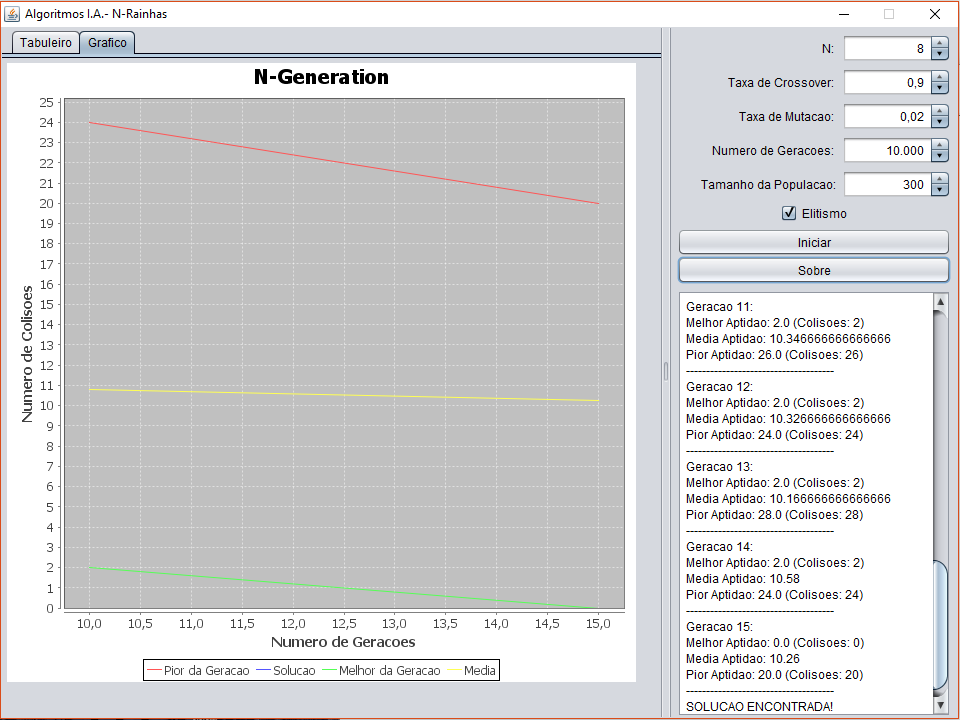
\includegraphics[width=14cm]{TELA02.png}
\end{figure}
\begin{figure}[!htb]
	\label{Figura 5}
	\centering
	\caption{População = 500}
	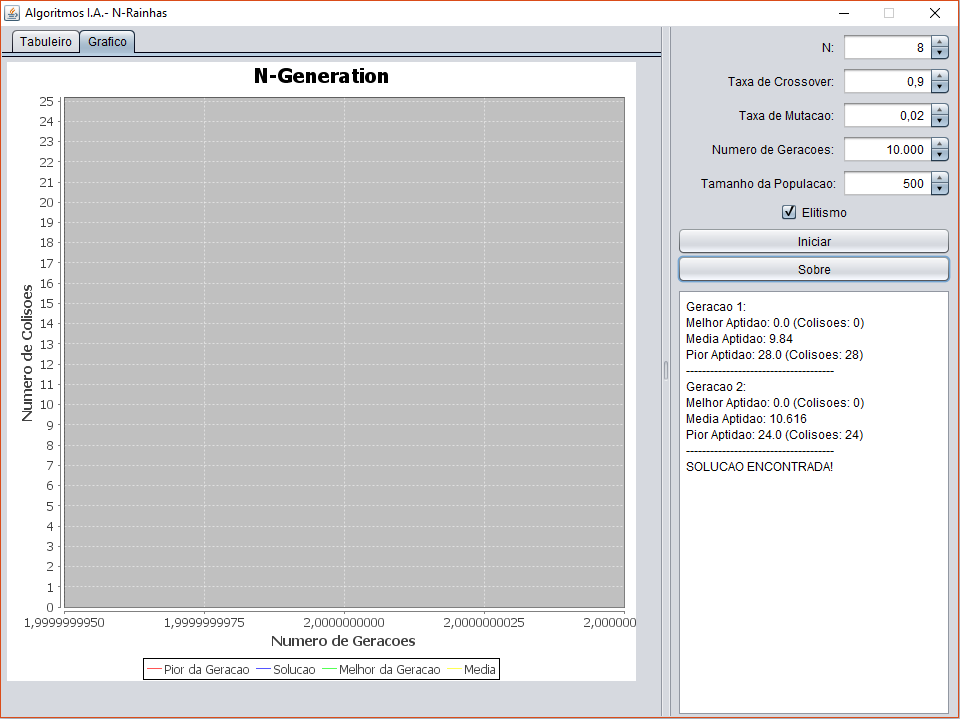
\includegraphics[width=14cm]{TELA03.png}
\end{figure}

\newpage
\thispagestyle{main}
\subsubsection{Variação do Crossover}

\begin{figure}[!htb]
	\label{Figura 6}
	\centering
	\caption{Crossover = 20\%}
	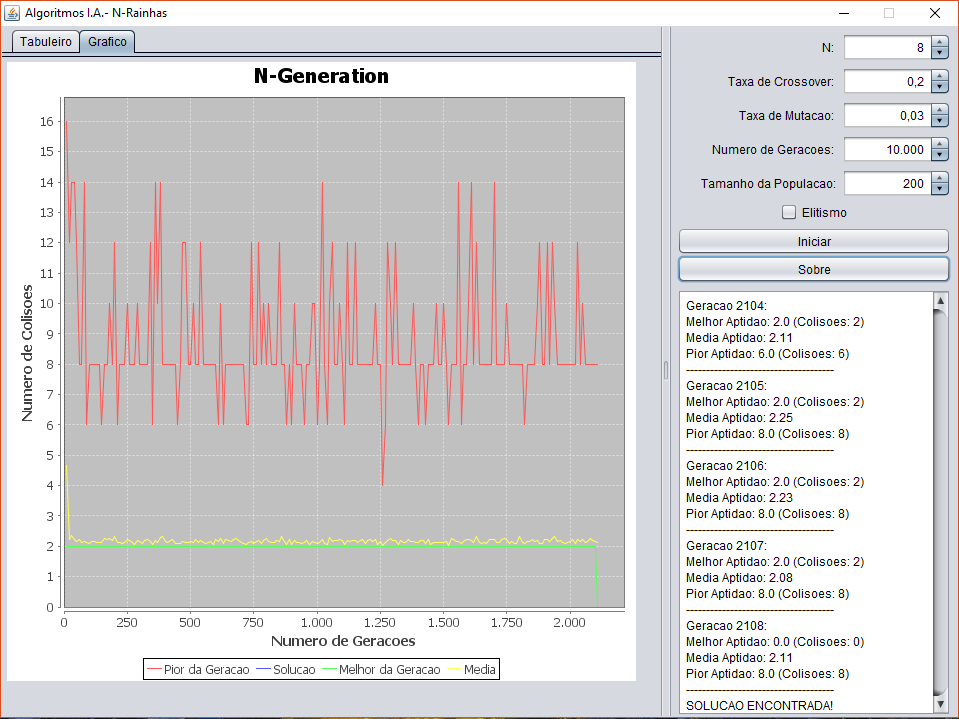
\includegraphics[width=14cm]{TELA04.png}
\end{figure}
\begin{figure}[!htb]
	\label{Figura 7}
	\centering
	\caption{Crossover = 50\%}
	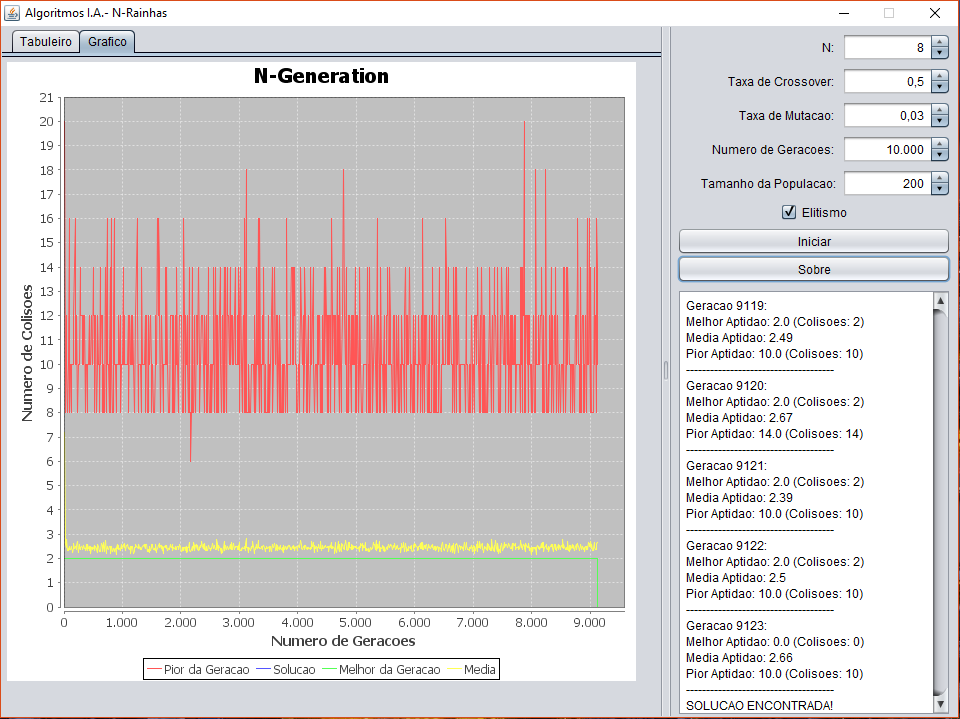
\includegraphics[width=14cm]{TELA05.png}
\end{figure}
\begin{figure}[!htb]
	\label{Figura 8}
	\centering
	\caption{Crossover = 80\%}
	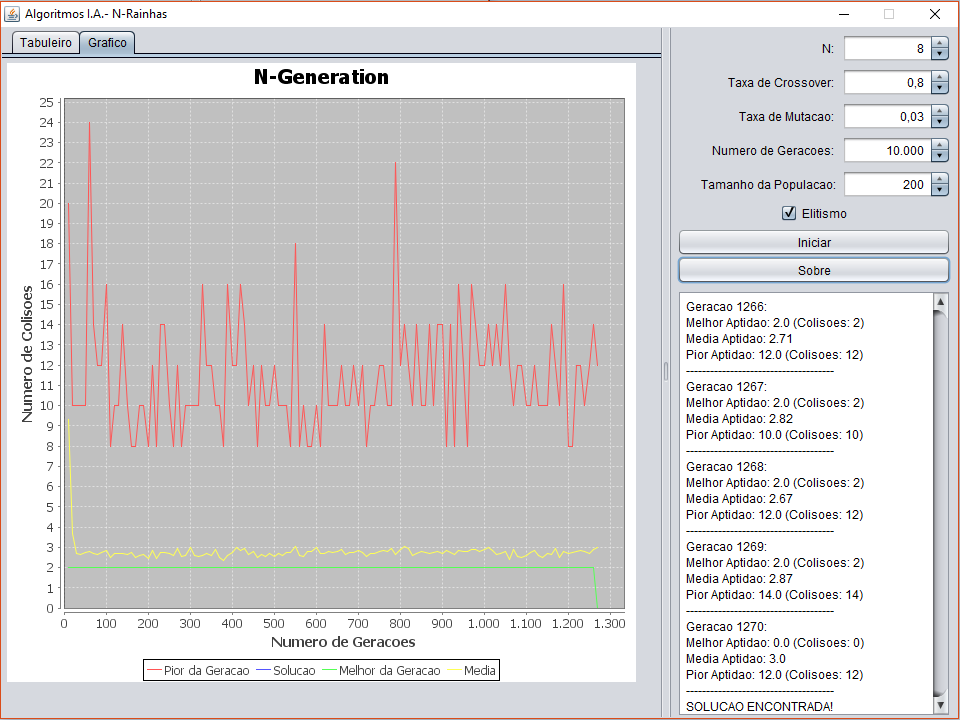
\includegraphics[width=14cm]{TELA06.png}
\end{figure}

\subsubsection{Variação da Mutação}

\begin{figure}[!htb]
	\label{Figura 6}
	\centering
	\caption{Mutação = 1\%}
	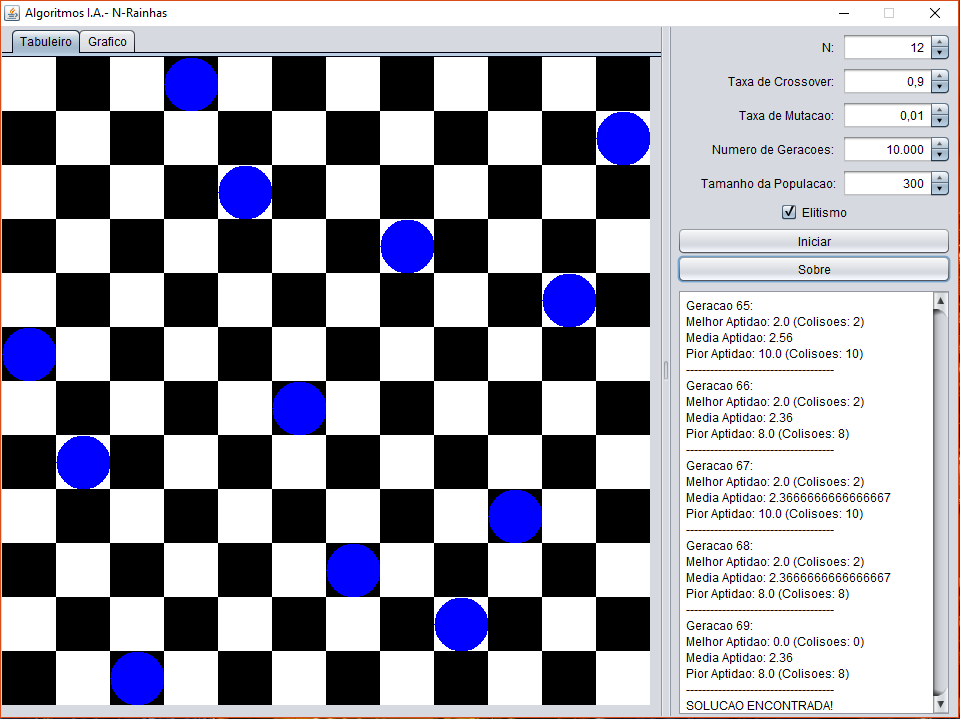
\includegraphics[width=14cm]{TELA07.png}
\end{figure}
\begin{figure}[!htb]
	\label{Figura 7}
	\centering
	\caption{Mutação = 10\%}
	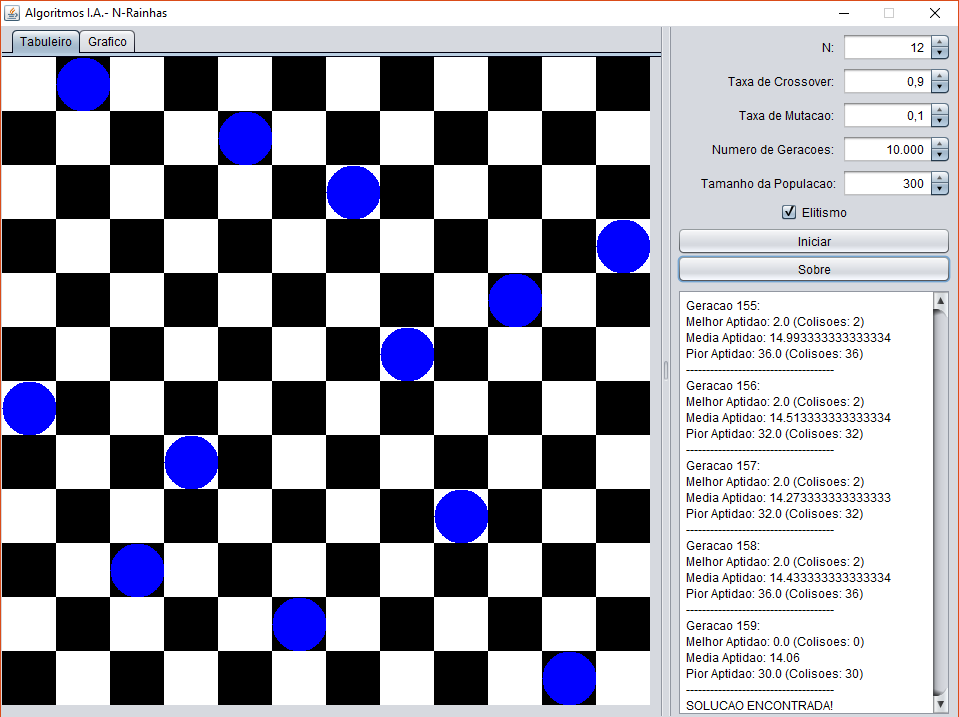
\includegraphics[width=14cm]{TELA08.png}
\end{figure}
\begin{figure}[!htb]
	\label{Figura 8}
	\centering
	\caption{Mutação = 50\%}
	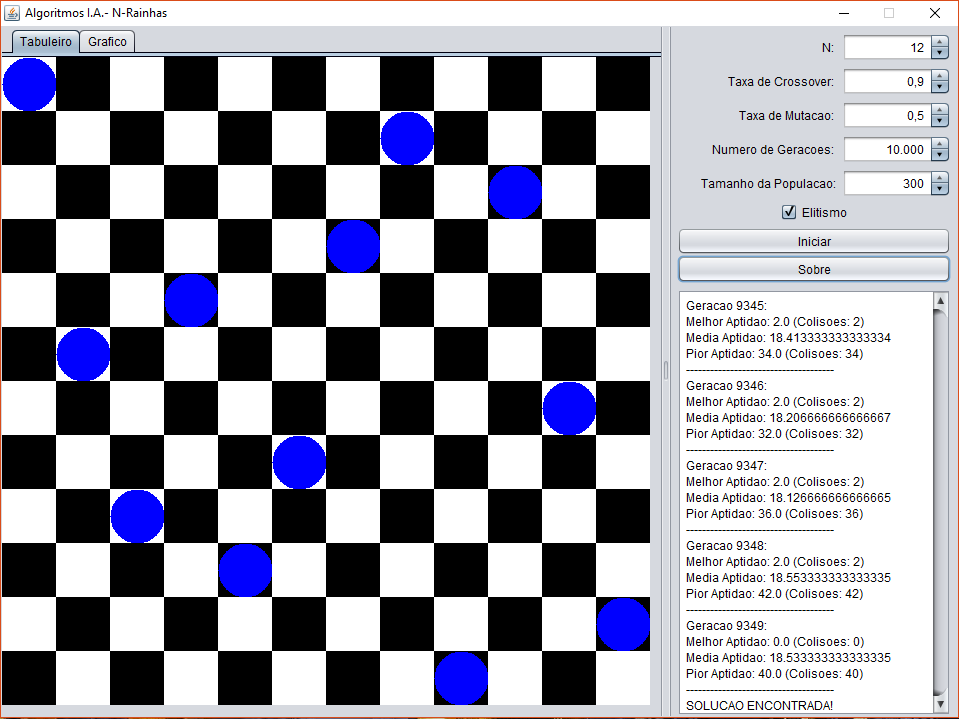
\includegraphics[width=14cm]{TELA09.png}
\end{figure}



\newpage
\thispagestyle{main}
\subsection{Considerações finais}

O uso e a aplicabilidade dos algoritmos genéticos realmente impressiona, a mecânica de sua implementação não é tão complexa (pelo menos no caso estudado) e os resultados são bem satisfatórios.

%%%%%%%%%%%% REFERÊNCIAS %%%%%%%%%%%%%
\newpage
\thispagestyle{main}

\addcontentsline{toc}{section}{REFERÊNCIAS}
\begin{flushleft}
{\large \textbf{REFERÊNCIAS}}\\
\vspace{0.5cm}

\hspace{4ex}FIRMINO, Manoel – Notas de Aula para Otimização de Sistemas, DCA-UFRN;\\
\vspace{0.8cm}
\hspace{4ex}GENÉTICOS, Algoritmos (AG's) - Prof.Von Zuben, DCA/FEEC/Unicamp. Disponível em: <ftp://ftp.dca.fee.unicamp.br/pub/docs/vonzuben/ia707\_01/topico6\_01.pdf>. Acessado em 7 de Abril de 2016;\\
\vspace{0.8cm}
\hspace{4ex}GENÉTICOS, Algoritmos - Instituto de Ciências Matemáticas e de Computação(ICMC) USP-São Carlos. Disponível em: <http://www.icmc.usp.br/pessoas/andre/research/genetic/>. Acessado em 8 de Abril de 2016;\\
\vspace{0.8cm}
\hspace{4ex}GENÉTICOS, Algoritmos - Wikipédia A enciclopédia livre. Disponível em: <https://pt.wikipedia.org/wiki/Algoritmo\_genético>. Acessado em 7 de Abril de 2016;\\
\vspace{0.8cm}
\hspace{4ex}LINDEN, Ricardo - Algoritmos genéticos: uma importante ferramenta de inteligência Computacional $2^a$ ed., Brasport,2008.\\
\vspace{0.8cm}

\end{flushleft}

\vspace{3cm}

%%%%%%%%%%%%%% ANEXOS %%%%%%%%%%%%%%%%
%\newpage
%\thispagestyle{main}
%
%\addcontentsline{toc}{section}{ANEXOS}
%\begin{flushleft}
%{\large \textbf{ANEXOS}}
%\end{flushleft}

%\vspace{3cm}

%
%%%%%%%%%%%%% APÊNDICES %%%%%%%%%%%%%%
%\newpage
%\thispagestyle{main}
%
%\addcontentsline{toc}{section}{APÊNDICES}
%\begin{flushleft}
%{\large \textbf{APÊNDICES}}
%\end{flushleft}
%
%\vspace{3cm}
%
%\begin{flushleft}
%\hspace{4ex}Documentos elaborados pelo próprio autor do trabalho que podem ser
%acrescentas no final do trabalho com a finalidade de documentar dados (algoritmos) ou
%fatos citados no decorrer de seu desenvolvimento. São documentos que complementam
%seu raciocínio sem, contudo, prejudicar a explanação realizada no corpo do trabalho.
%\end{flushleft}

\end{document}